\begin{figure}
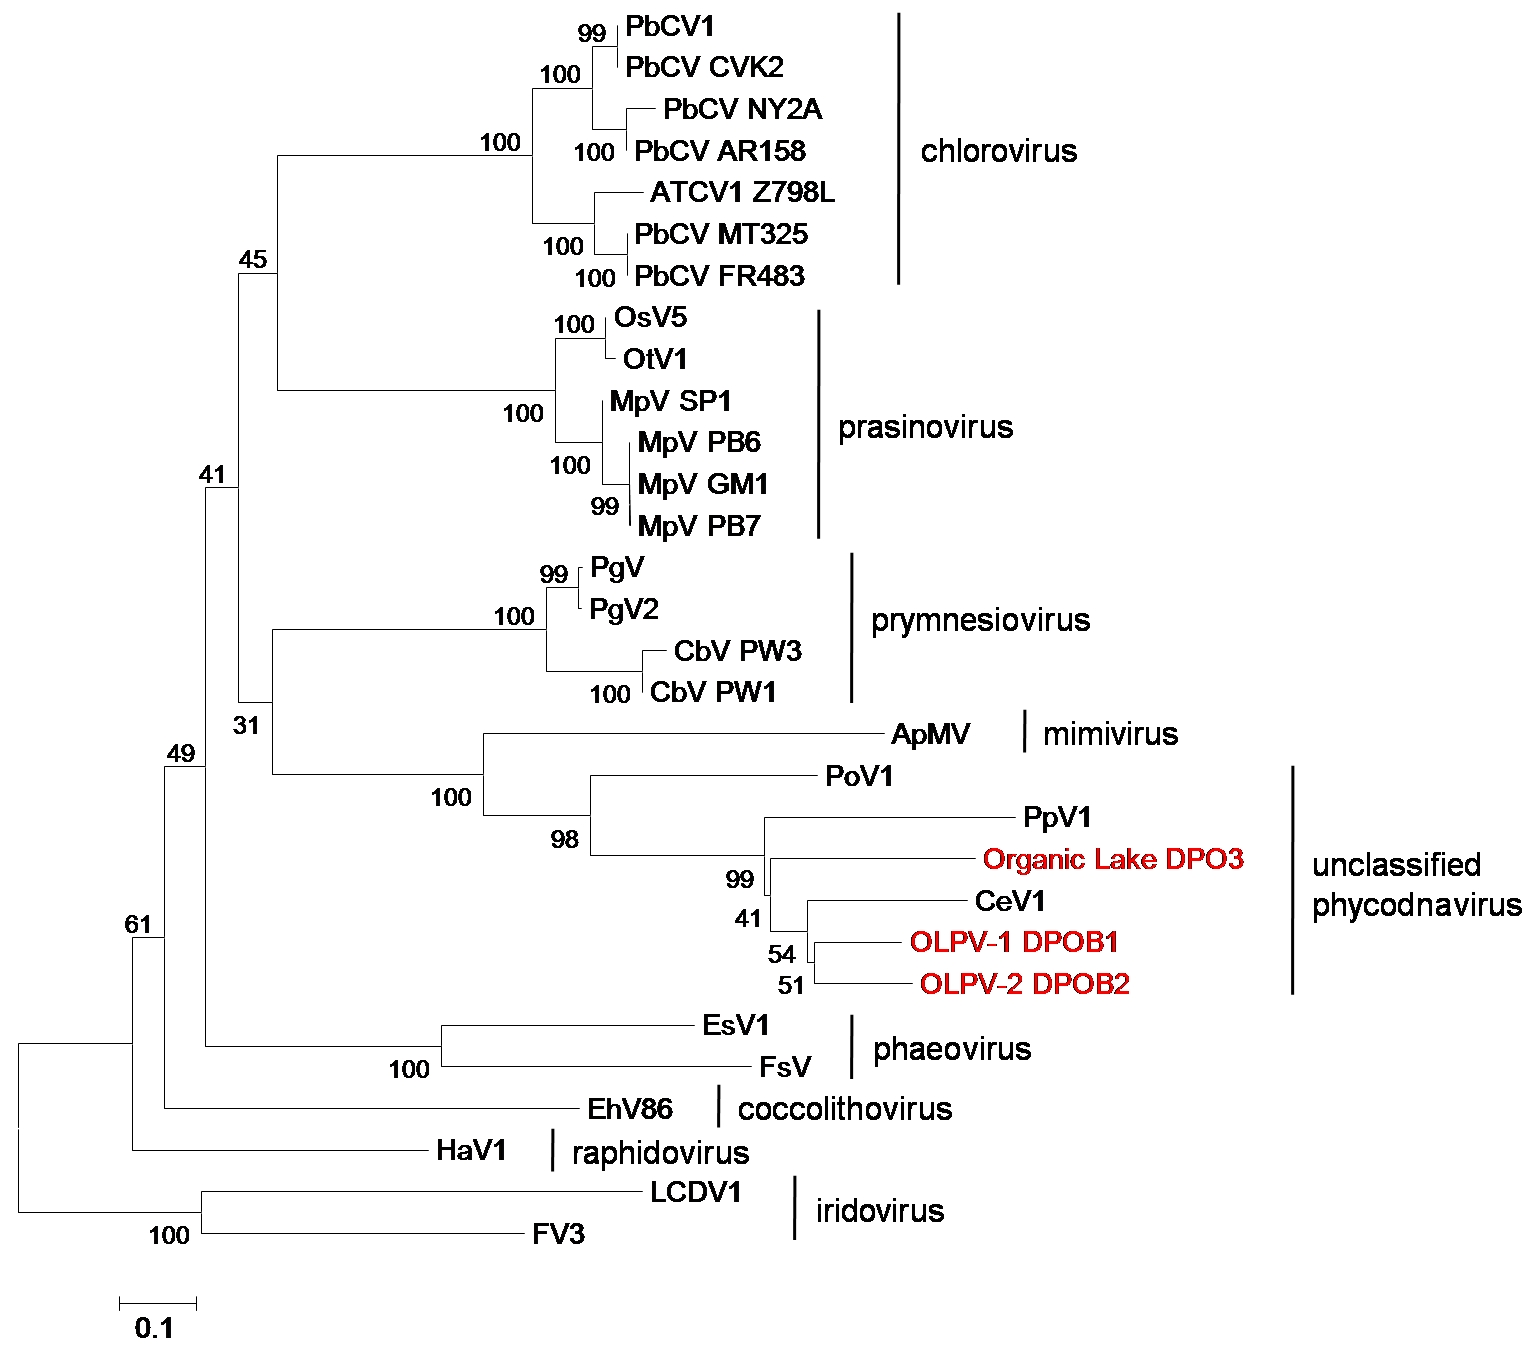
\includegraphics[width=\textwidth]{olv_figures/OLPV_full_dpo.jpg}
\caption[Phylogeny of \acs{OLPV} B family DNA polymerase sequences]{Neighbour-joining tree of B family DNA polymerase amino acid sequences from \acs{OLPV} and \acs{NCLDV} sequences from GenBank. 
Organic Lake sequences are shown in red.
Abbreviations and accession numbers from bottom to top: PbCV1, \emph{Paramecium bursaria} chlorella virus 1 (AAC00532.1); PbCV CVK2, \emph{P. bursaria} chlorella virus CVK2 (BAA35142.1); PbCV NY2A,  \emph{P. bursaria} chlorella virus NY2A (ABT14648.1); PbCV AR158, \emph{P. bursaria} chlorella virus AR158 (ABU43776.1); AtCV1, \emph{Acathocystis turfacea} chlorella virus (ABT16932.1); PbCV MT325,  \emph{P. bursaria} chlorella virus MT325(ABT13573.1); PbCV FR483, \emph{P. bursaria} chlorella virus FR483 (ABT15308.1); OsV5, \emph{Ostreococcus} virus 5 (ABY28020.1); OtV1, \emph{O. tauri} virus 1(YP\_003495047.1);  MpV SP1, \emph{Micromonas pusilla} virus SP1(AAB66713.1); MpV PB6, \emph{M. pusilla} virus PB6 (AAB49743.1); MpV GM1, \emph{M. pusilla} virus GM1 (AAB49742.1); MpV PB7, \emph{M. pusilla} virus PB7 (AAB49744.1); CbV PW1, \emph{Chrysochromulina brevifilum} virus PW1 (AAB49739.1); CbV PW3, \emph{C. brevifilum} virus PW3 (AAB49740.1); ApMV, \emph{Acathamoeba polyphaga} mimivirus (AAV50591.1); PoV,  \emph{Pyramimonas orientalis} virus (ABU23717.1); PpV, \emph{Phaeocystis pouchetii} virus (ABU23718.1); CeV1, \emph{C. ericinia} virus 1 (ABU23716.1); EsV1, \emph{Ectocarpus silicolosus} virus (AAK14511.1); FsV, \emph{Feldmannia} sp. virus (AAB67116.1); EhV86, \emph{Emiliania huxleyii} virus 86 (CAI65453.1); HaV1, \emph{Heterosigma akashiwo} virus 1 (BAE06251.1); FV3, Frog virus 3 (AAT09720.1) and LCDV1, Lymphocystis disease virus 1 (NP\_078724.1). 
}
\label{fig:OLPV_full_dpo}

\end{figure}
